%%%%%%%%%%%%%%%%%%%%%%%%%%%%%%%%%%%%%%%%%
% 王艺霏中文 CV
% 基于 ModernCV 模板，使用 XeLaTeX 编译
%%%%%%%%%%%%%%%%%%%%%%%%%%%%%%%%%%%%%%%%%

\documentclass[10pt,a4paper,sans]{moderncv}

% 中文与版式
\usepackage[UTF8,fontset=fandol]{ctex}
\usepackage{graphicx}
\usepackage{enumitem}
\usepackage[scale=0.86]{geometry}

\moderncvstyle[nosymbols]{classic}
\moderncvcolor{orange}
\colorlet{bodyrulecolor}{color1}
\colorlet{bodyrulecolor}{color1}
\colorlet{sectioncolor}{color1}
\colorlet{subsectioncolor}{color1}
\nopagenumbers

\setlength{\hintscolumnwidth}{2.4cm}
\setlist[itemize]{
  leftmargin=1.5em,
  itemsep=0.15em,
  topsep=0.2em,
  parsep=0pt,
  partopsep=0pt
}

% 个人信息
\firstname{Yifei Wang}
\familyname{}
\title{北京理工大学}
\mobile{18213820019}
\email{1120243123@bit.edu.cn}
\homepage{sophie618.github.io}
\extrainfo{
  \href{mailto:3441606266@qq.com}{3441606266@qq.com}
  \quad
  \href{https://github.com/Sophie618}{github.com/Sophie618}
}
\photo[72pt][0pt]{moderncv-cn-assets/photo.jpeg}

\begin{document}

\makecvtitle
\vspace{-1.2em}

%----------------------------------------------------------------------------------------
% 教育背景
%----------------------------------------------------------------------------------------

\section{教育背景}

\cventry
  {2024.09--至今}
  {计算机科学与技术专业 · 徐特立英才班}
  {北京理工大学}
  {工学学士在读}
  {}
  {
    \begin{itemize}
      \item 徐特立英才班教学班班长；
      \item CET-4：572；全国大学生英语竞赛二等奖。
    \end{itemize}
  }

%----------------------------------------------------------------------------------------
% 研究兴趣
%----------------------------------------------------------------------------------------

\section{研究兴趣}

\cvitem{自适应智能体}{
  强化学习与长期记忆、长程交互中的学习和决策
}
\cvitem{模型自进化}{
  递归学习、反馈驱动的自我改进与能力演化
}
\cvitem{多模态智能}{
  多模态基础模型、智能体系统、模型可解释性及脑—模型语义对齐
}

%----------------------------------------------------------------------------------------
% 科研经历
%----------------------------------------------------------------------------------------

\section{科研经历}

\cventry
  {2025.12--2026.05}
  {Threader：面向对话智能体的长期记忆}
  {清华大学科研合作}
  {共同作者}
  {2026 NeurIPS在投}
  {
    \begin{itemize}
      \item 针对传统对话智能体压缩式记忆存在的信息丢失、高延迟和高成本问题，
      设计并实现无损长效记忆框架Threader。
      \item 提出“主题分割＋多视角编码＋多信号检索”范式，
      摒弃依赖大语言模型的摘要压缩流程；
      在对话记忆任务中实现100\%信息保留，
      构建速度提升一个数量级，并大幅降低Token成本。
      \item 在多个长对话记忆基准上全面超越MemGPT、Mem0等主流SOTA模型，
      显著提升智能体的长程对话一致性与响应效率。
    \end{itemize}
  }

\cventry
  {2025.09--2026.05}
  {SAIL：脑—模型语义对齐}
  {北京理工大学}
  {共同作者}
  {2026 NeurIPS在投}
  {
    \begin{itemize}
      \item 针对多模态大模型（MLLM）内部表征纠缠、可解释性差的问题，
      构建基于稀疏自编码器（SAE）的脑—模型语义对齐框架SAIL。
      \item 通过SAE将高维视觉特征解纠缠为单语义概念原子，
      并与人类视觉皮层fMRI信号精准匹配，
      揭示MLLM与腹侧视觉通路的层级对应关系。
      \item 实验表明，SAE提取的特征相较原始模型特征，
      在人脑对齐任务上的性能提升显著，
      为多模态模型可解释性研究提供了新的范式。
    \end{itemize}
  }

%----------------------------------------------------------------------------------------
% 实习经历
%----------------------------------------------------------------------------------------

\section{实习经历}

\cventry
  {2026.04--2026.06}
  {产品解决方案实习生}
  {字节跳动 · 火山方舟}
  {北京}
  {AI产品与MaaS解决方案}
  {
    \begin{itemize}
      \item 参与企业级AI产品与MaaS解决方案设计，
      梳理基础模型能力、业务场景与产品落地路径。
      \item 支持ToB AI场景的解决方案调研与产品沟通，
      将技术能力转化为可执行的业务方案。
    \end{itemize}
  }

%----------------------------------------------------------------------------------------
% 项目经历
%----------------------------------------------------------------------------------------

\clearpage
\section{项目经历}

\cventry
  {2025.11--至今}
  {Multi-Agent：基于MCP协议的电商智能助手平台}
  {\href{https://github.com/Sophie618/Multi-Agent}{GitHub}}
  {}
  {重构中}
  {
    \begin{itemize}
      \item 探索Anthropic发布的模型上下文协议（MCP），
      构建连接大语言模型与Medusa电商后台的智能中介系统。
      \item 搭建标准MCP Server，
      使大语言模型通过通用协议自动发现并调用
      \texttt{search\_products}、\texttt{get\_details}等工具。
      \item 探索Planner--Worker多智能体协作架构，并结合RAG增强任务处理。
      \item 实现“用户请求$\rightarrow$Claude大语言模型$\rightarrow$路由器
      $\rightarrow$MCP Server$\rightarrow$后端API”的完整数据链路，
      验证大语言模型操作外部系统的可行性。
      \item 使用Vue 3构建对话界面，
      解析工具执行结果并渲染为可视化商品卡片；
      项目正由单Agent向Multi-Agent架构演进。
    \end{itemize}
  }

\cventry
  {2026.01}
  {Collector+（Collector-AI）：基于线性单体架构的低延迟信息提取助手}
  {\href{https://github.com/Sophie618/Creator_ai}{GitHub}；
  \href{https://collectorai.top/}{在线演示}}
  {}
  {}
  {
    \begin{itemize}
      \item 通过大语言模型将长文本或视频快速转化为二元预测性问题，
      实现“游戏化阅读”（Gamified Reading）。
      \item 摒弃复杂的Agent编排，
      设计Linear Monolithic线性单体架构并结合FastAPI异步处理，
      将端到端生成延迟压缩至15--30秒。
      \item 设计认知科学家System Prompt，
      在单次推理中通过Chain-of-Thought完成内容重构、
      反直觉观点挖掘与格式化输出。
      \item 实现微信公众号、哔哩哔哩通用内容解析器，
      以及动态渲染页面的通用解析，
      解决懒加载和动态渲染问题；
      使用React Context管理全局状态，构建直觉对赌交互机制。
    \end{itemize}
  }

\cventry
  {2025.12}
  {FitSnap：基于视频语义理解的结构化指令生成系统}
  {\href{https://fit-snap-beige.vercel.app/}{在线演示}}
  {}
  {私有仓库，可提供技术报告}
  {
    \begin{itemize}
      \item 面向人类学习场景中非结构化视频难以被执行的问题，
      构建将长视频实时转化为结构化步骤指令的系统。
      \item 使用Python抓取哔哩哔哩视频字幕与元数据，
      构建“视频—文本—指令”映射管道；
      利用DeepSeek-V3进行长文本语义理解，
      开发内容无关的提取算法，自动过滤冗余信息并归纳核心操作。
      \item 通过System Prompt约束模型输出严格JSON格式，
      包含时间戳、操作分类和关键参数，
      实现从流式媒体到结构化指令的跨维度转换。
      \item 使用Next.js 16、React 19和Zustand构建前端，
      完成视频时间戳与步骤卡片的双向实时联动，
      并按健身、烹饪等任务动态生成领域界面。
    \end{itemize}
  }

\cventry
  {2024.09--2025.10}
  {BiGEM数据检索与可视化平台}
  {\href{https://gitlab.igem.org/2025/software-tools/bit-china}{GitLab源码}}
  {}
  {\href{https://2025.igem.wiki/bit-china/}{项目Wiki}}
  {
    \begin{itemize}
      \item 获2025 iGEM国际金奖及全球本科生组Best Software奖，
      并正向上申报软件著作权。
      \item 面向2004--2024年合成生物学竞赛数据，
      使用Python爬虫完成海量科研数据清洗；
      基于D3.js和Three.js实现力导向图、桑基图和树状关系图的动态渲染，
      揭示全球队伍间的合作网络。
      \item 接入大模型API，对生物元件库进行语义分析，
      实现超越关键词匹配的模糊扩展搜索，
      提升科研数据检索效率。
    \end{itemize}
    % 作品集版本可取消以下注释：
    % \begin{center}
    %   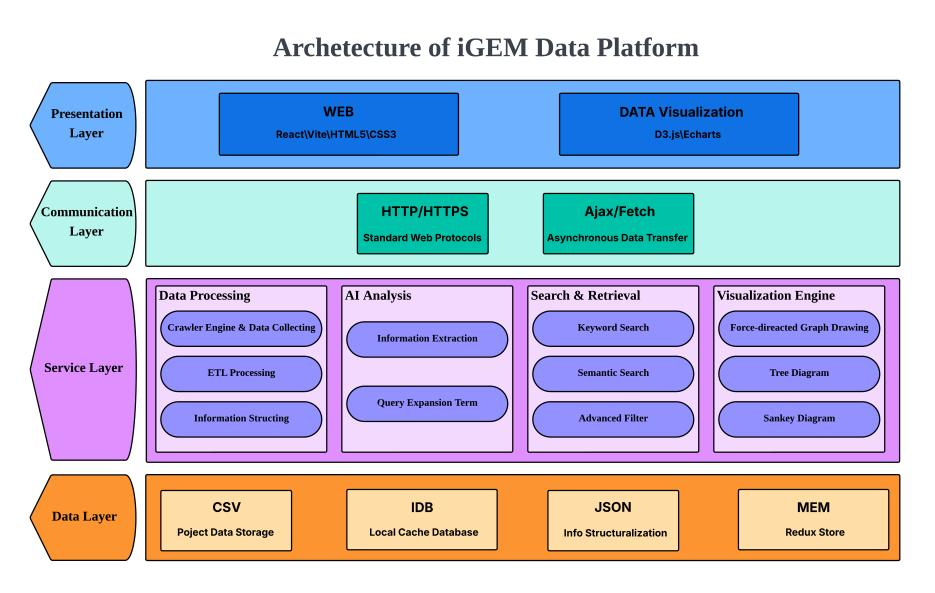
\includegraphics[width=0.82\linewidth]{moderncv-cn-assets/bigem-architecture.png}
    % \end{center}
  }

%----------------------------------------------------------------------------------------
% 专业技能
%----------------------------------------------------------------------------------------

\section{专业技能}

\cvitem{编程学习}{Python、PyTorch、TypeScript}
\cvitem{开发技能}{React、Git}
\cvitem{语言能力}{中文（母语）；英语（流利）}

%----------------------------------------------------------------------------------------
% 荣誉与奖项
%----------------------------------------------------------------------------------------

\section{荣誉与奖项}

\cvitem{2026}{
  美国大学生数学建模竞赛H奖
}
\cvitem{2025}{
  iGEM国际遗传工程机器设计竞赛国际金奖；
  全球本科生组Best Software奖
}
\cvitem{2025}{
  全国大学生数学建模竞赛北京市一等奖
}

\cvitem{2025}{
  全国大学生英语竞赛二等奖
}
\end{document}
